\chapter{}
In this chapter the interfaces between the different subsystems are discussed. In section \ref{sec:n2chart} the interfaces are shown in a $N^2$ chart. 

\section{$N^2$ Chart}
\label{sec:n2chart}
The $N^2$ chart shows the interfaces between the different functions of the system. The chart could be found in figure \ref{fig:n2chart} on page \pageref{fig:n2chart}. The functions are in the dark grey boxes, while the interactions are shown by the dotted boxes and move clockwise. The system is split up in the emitter satellite, a receiver satellite and the ground segment, denoted by the large bold boxes. Outside of these boxes is the outside world, e.g. the Sun and customers. The starred interactions dependent on the level of communication centralisation.

The basic workings of the system is that the laser sends down a laser pulse, which is reflected by the Earth and received by receivers in the receiver satellites and the main satellite. Combined with the time from the navigation subsystem the photon counts are stored in the data storage. The communication subsystem sends down the data to be received by the ground station. Before a laser pulse can be send or received the satellites need to be pointed by the attitude control subsystem and the pointing mechanism. The current attitude is determined by the attitude determination subsystem. The \ac{EPS} subsystem provides power to all other subsystems. 

\begin{figure}
\centering
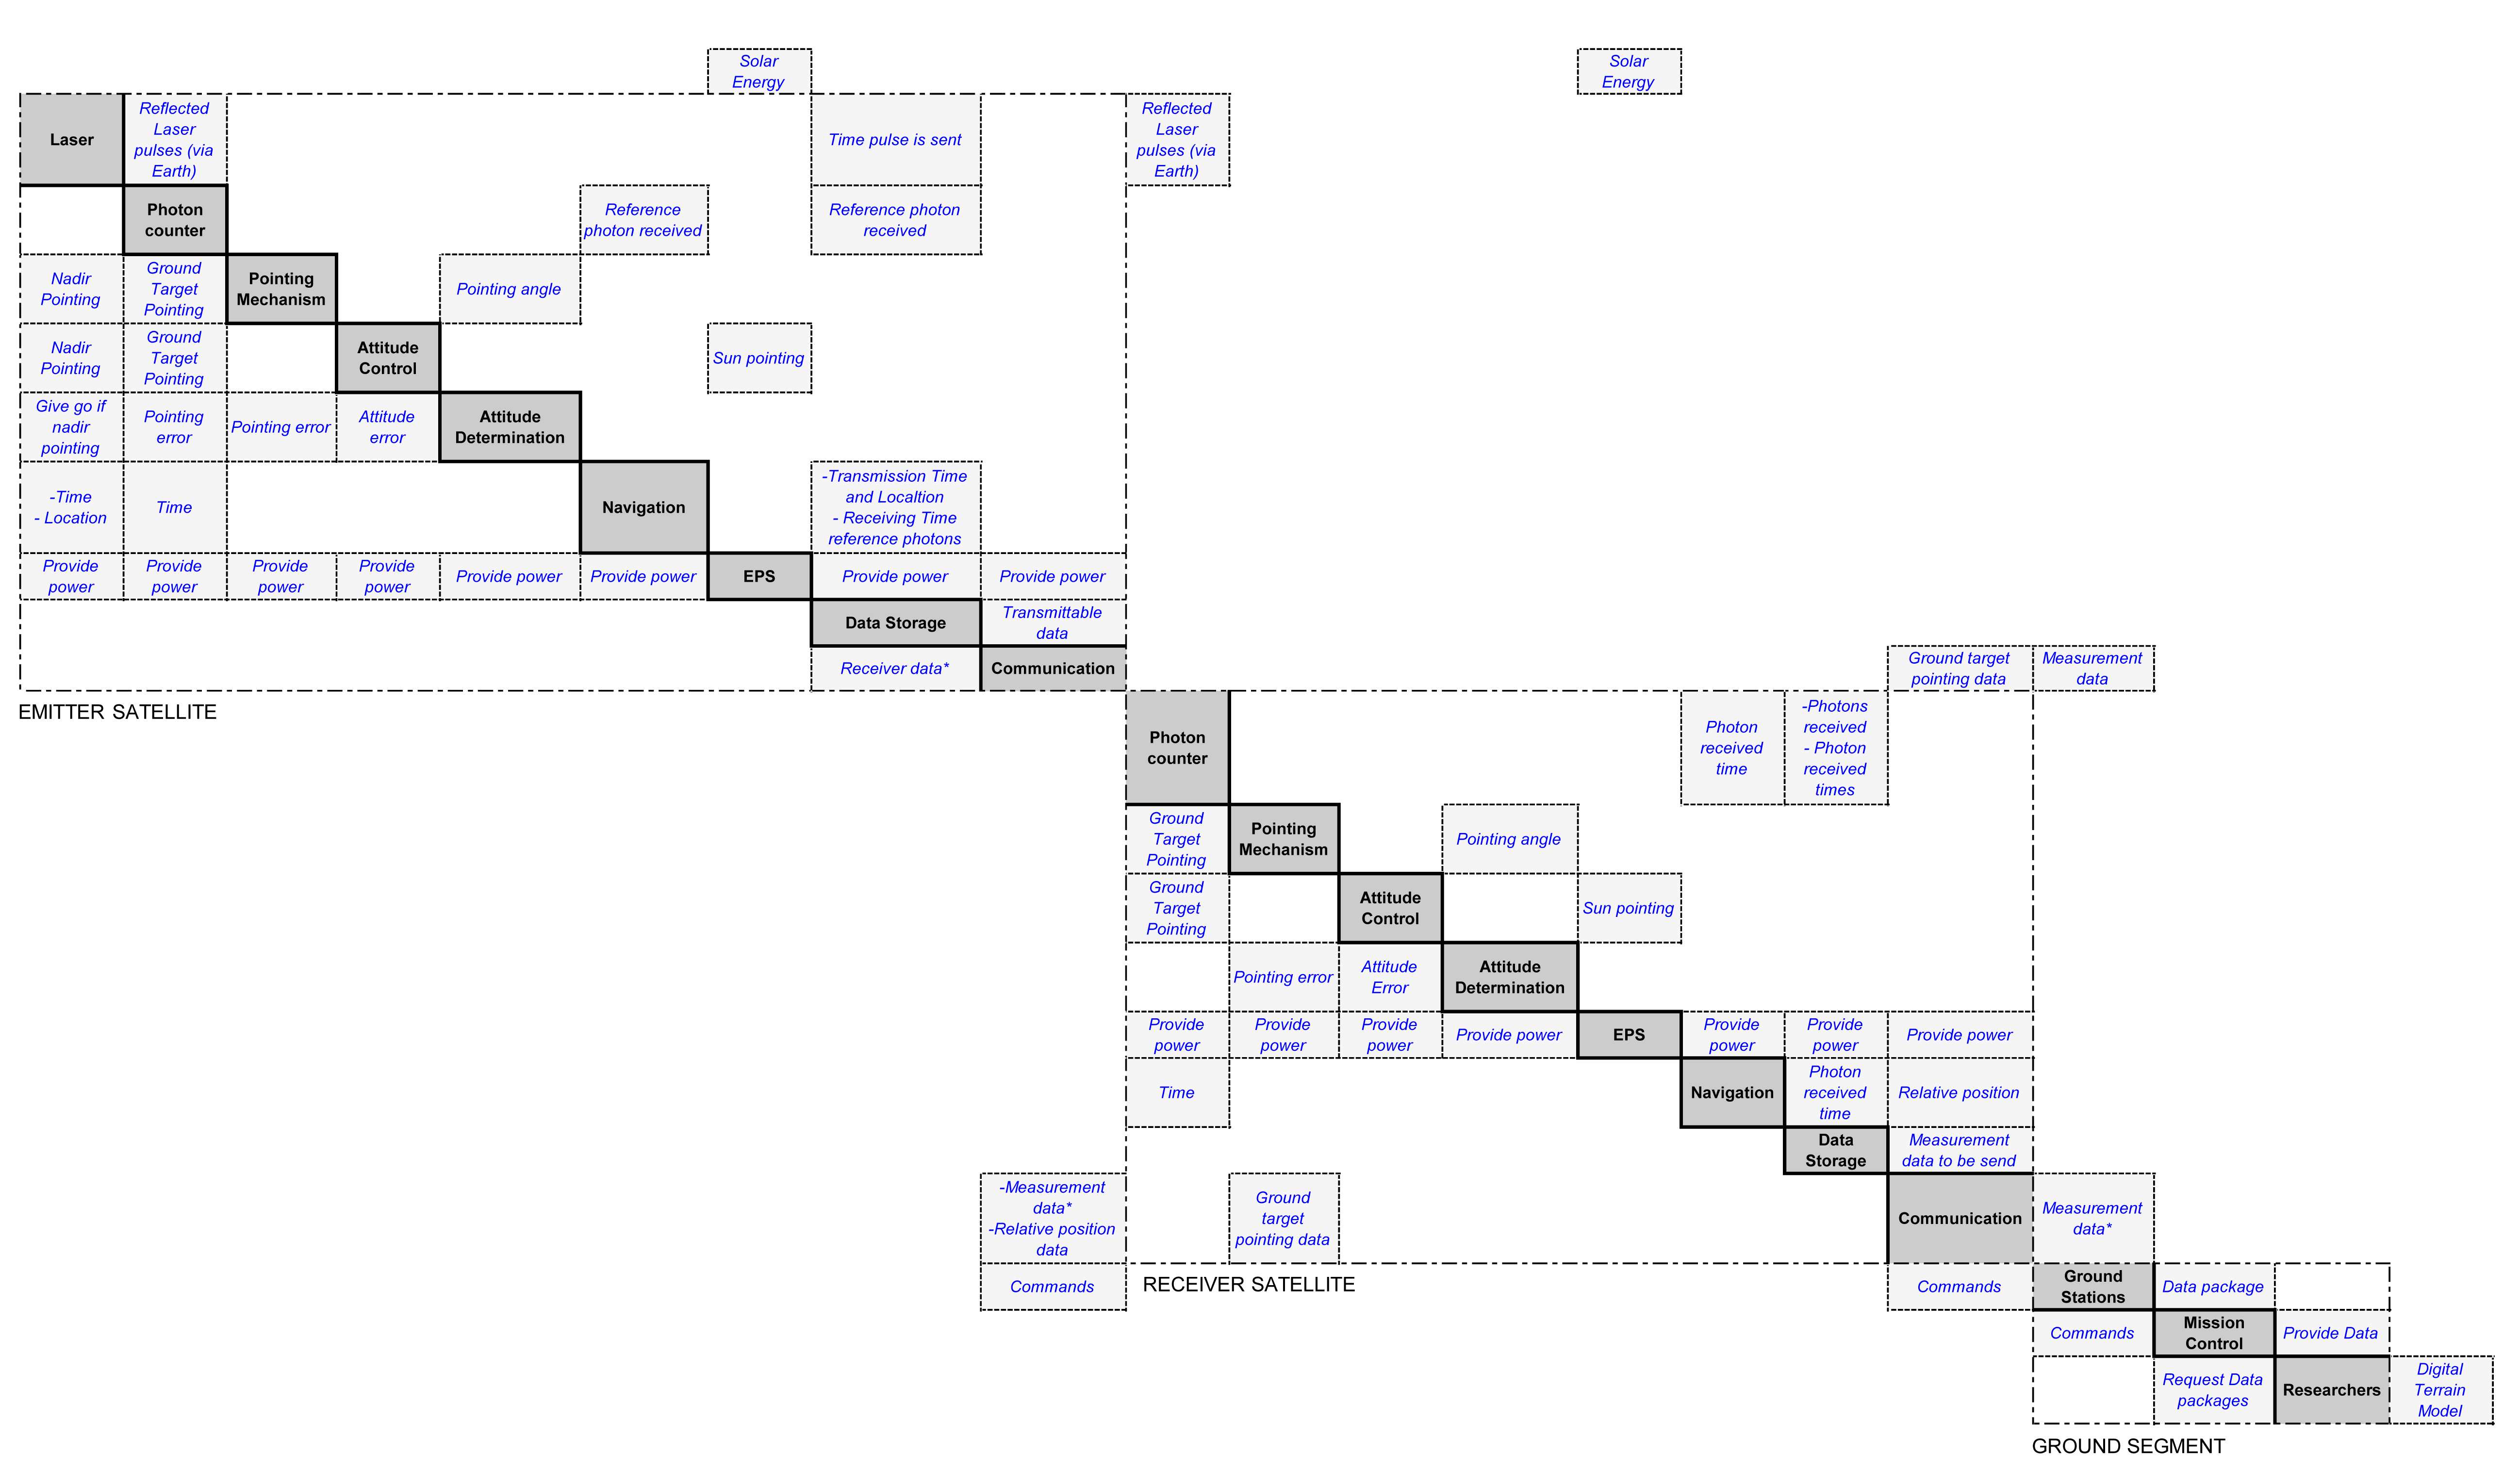
\includegraphics[angle = 90, width = 0.7\textwidth, bb= 0 0 3421px 1861px]{img/N2chart_wo.png} 
\caption{$N^2$ chart of the Laser Swarm mission}
\label{fig:n2chart}
\end{figure}